% BIDS-Eye project page, Figure 1: one question traced through the query pipeline.
% State of 2026-11-15. The SQL in stage 3 is the output of
% backend/services/participant_query_compiler.py for the plan in stage 1 (shortened).
% Layout after the overview figures of Ferber et al. (arXiv 2404.04667, 2407.13463):
% one pale panel, numbered steps as text, the concrete artefact under each step.
% Build:  ./build-paper-figures.sh
\documentclass[tikz,border=6pt]{standalone}
\usepackage[T1]{fontenc}
\usepackage[default,semibold]{sourcesanspro}
\usepackage[scaled=0.86]{sourcecodepro}
\usepackage{textcomp}
\usepackage{amssymb}
\usetikzlibrary{arrows.meta,positioning,calc,backgrounds,shapes.geometric,shapes.callouts}

\definecolor{ink}{HTML}{1B1F24}
\definecolor{mute}{HTML}{5C646E}
\definecolor{rule}{HTML}{8D95A0}
\definecolor{panel}{HTML}{F4F5F7}
\definecolor{card}{HTML}{FFFFFF}
\definecolor{cardB}{HTML}{D5D9DF}
\definecolor{llm}{HTML}{5B45C0}  \definecolor{llmF}{HTML}{E9E4FA}
\definecolor{cod}{HTML}{2B5C9E}  \definecolor{codF}{HTML}{DFE9F7}
\definecolor{dat}{HTML}{9A6A08}  \definecolor{datF}{HTML}{FAEFD2}
\definecolor{con}{HTML}{17704C}  \definecolor{conF}{HTML}{DDF1E6}
\definecolor{pro}{HTML}{94660A}  \definecolor{proF}{HTML}{FAEFD2}
\definecolor{ctr}{HTML}{B03A2E}  \definecolor{ctrF}{HTML}{FAE3E0}
\definecolor{hl}{HTML}{FFE9A8}

\newcommand{\sbf}[1]{{\fontseries{sb}\selectfont #1}}
\newcommand{\mono}[1]{{\ttfamily #1}}
\newcommand{\hlt}[1]{\colorbox{hl}{\vphantom{(g}#1}}
\newcommand{\key}[1]{{\color{cod}#1}}
\newcommand{\str}[1]{{\color{con}#1}}
\newcommand{\dd}{{\color{rule}\dots}}
\newcommand{\tick}{{\color{con}\checkmark}}

\begin{document}
\hyphenpenalty=10000 \exhyphenpenalty=10000
\setlength{\fboxsep}{1.2pt}
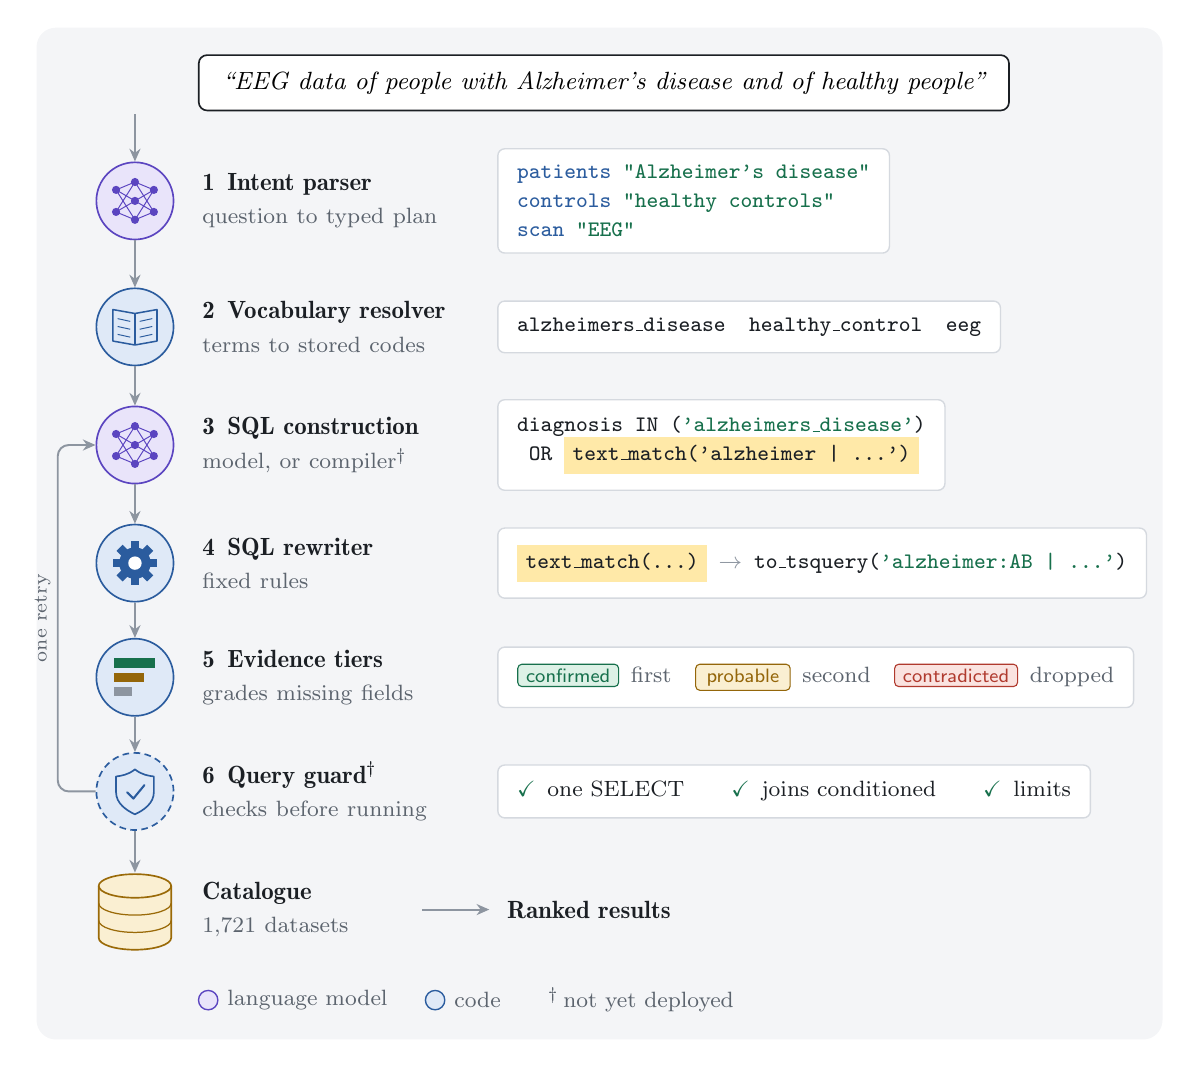
\begin{tikzpicture}[
  font=\small\color{ink},
  >={Stealth[length=4.6pt,width=4pt]},
  flow/.style={->, draw=rule, line width=0.7pt},
  badge/.style={circle, draw=#1, fill=#1F, line width=0.6pt, minimum size=0.98cm, inner sep=0pt},
  sname/.style={anchor=west, inner sep=0pt, align=left, text width=3.5cm},
  acard/.style={anchor=west, draw=cardB, fill=card, line width=0.5pt, rounded corners=2.5pt,
               inner xsep=7pt, inner ysep=6pt, align=left, 
               font=\ttfamily\fontsize{7.6}{10.4}\selectfont\color{ink}},
  stag/.style={font=\fontsize{6.8}{8}\selectfont\fontseries{sb}\selectfont\color{#1}, fill=#1F,
              rounded corners=1.5pt, inner xsep=3.2pt, inner ysep=1.8pt, anchor=west},
  pill/.style={font=\fontsize{6.8}{8}\selectfont\sffamily\color{#1}, draw=#1, fill=#1F, line width=0.4pt,
               rounded corners=1.5pt, inner xsep=3pt, inner ysep=1.6pt, minimum width=1.2cm},
  % ── glyphs: what each stage is ──
  net/.pic={
    \foreach \a/\b in {-0.14/0.24,-0.14/0,-0.14/-0.24,0.14/0.24,0.14/0,0.14/-0.24}{
      \draw[line width=0.35pt] (-0.24,\a) -- (0,\b);
      \draw[line width=0.35pt] (0,\b) -- (0.24,\a);}
    \foreach \p in {(-0.24,0.14),(-0.24,-0.14),(0,0.24),(0,0),(0,-0.24),(0.24,0.14),(0.24,-0.14)}
      \fill \p circle (0.052);},
  book/.pic={
    \draw[line width=0.55pt, line join=round] (0,0.17) -- (-0.28,0.22) -- (-0.28,-0.18) -- (0,-0.23) -- (0.28,-0.18) -- (0.28,0.22) -- cycle;
    \draw[line width=0.55pt] (0,0.17) -- (0,-0.23);
    \foreach \y in {0.07,-0.03,-0.13}{
      \draw[line width=0.35pt] (-0.22,\y+0.035) -- (-0.06,\y);
      \draw[line width=0.35pt] (0.22,\y+0.035) -- (0.06,\y);}},
  gear/.pic={
    \foreach \a in {0,45,...,315} \fill[rotate=\a] (-0.055,0.15) rectangle (0.055,0.275);
    \fill (0,0) circle (0.2);
    \fill[white] (0,0) circle (0.085);},
  tiers/.pic={
    \fill[con] (-0.26,0.12) rectangle (0.26,0.24);
    \fill[pro] (-0.26,-0.06) rectangle (0.12,0.06);
    \fill[rule] (-0.26,-0.24) rectangle (-0.04,-0.12);},
  shield/.pic={
    \draw[line width=0.6pt, line join=round]
      (0,0.28) .. controls (0.09,0.21) and (0.17,0.2) .. (0.24,0.19) -- (0.24,-0.01)
      .. controls (0.24,-0.15) and (0.11,-0.24) .. (0,-0.29)
      .. controls (-0.11,-0.24) and (-0.24,-0.15) .. (-0.24,-0.01) -- (-0.24,0.19)
      .. controls (-0.17,0.2) and (-0.09,0.21) .. cycle;
    \draw[line width=0.75pt, line cap=round, line join=round] (-0.1,-0.01) -- (-0.02,-0.09) -- (0.12,0.08);},
]
\def\xr{0.95}   % rail
\def\xn{1.8}    % stage names
\def\xc{5.55}   % artefacts
\newcommand{\gl}[1]{\\[1pt]{\footnotesize\color{mute}#1}}
\newcommand{\ar}{\enspace{\color{rule}$\rightarrow$}\enspace}

% ── Question ────────────────────────────────────────────────────────────────
\node[draw=ink, fill=card, line width=0.6pt, rounded corners=3pt, inner xsep=8pt, inner ysep=6pt,
      anchor=west, font=\small\itshape] (q) at (\xn-0.05,0.15)
  {``EEG data of people with Alzheimer's disease and of healthy people''};

% ── Stages: badge, name, what it produces ───────────────────────────────────
\node[badge=llm] (b1) at (\xr,-1.35) {}; \pic[llm] at (b1) {net};
\node[sname] at (\xn,-1.35) {\sbf{1\enspace Intent parser}\gl{question to typed plan}};
\node[acard] at (\xc,-1.35) {%
\key{patients}\enspace\str{"Alzheimer's disease"}\\
\key{controls}\enspace\str{"healthy controls"}\\
\key{scan}\enspace\str{"EEG"}};

\node[badge=cod] (b2) at (\xr,-2.95) {}; \pic[cod] at (b2) {book};
\node[sname] at (\xn,-2.95) {\sbf{2\enspace Vocabulary resolver}\gl{terms to stored codes}};
\node[acard] at (\xc,-2.95) {alzheimers\_disease\quad healthy\_control\quad eeg};

\node[badge=llm] (b3) at (\xr,-4.45) {}; \pic[llm] at (b3) {net};
\node[sname] at (\xn,-4.45) {\sbf{3\enspace SQL construction}\gl{model, or compiler\textsuperscript{\textdagger}}};
\node[acard] at (\xc,-4.45) {%
diagnosis IN (\str{'alzheimers\_disease'})\\
\enspace OR \hlt{text\_match('alzheimer | \dots')}};

\node[badge=cod] (b4) at (\xr,-5.95) {}; \pic[cod] at (b4) {gear};
\node[sname] at (\xn,-5.95) {\sbf{4\enspace SQL rewriter}\gl{fixed rules}};
\node[acard] at (\xc,-5.95) {\hlt{text\_match(\dots)}\ar to\_tsquery(\str{'alzheimer:AB | \dots'})};

\node[badge=cod] (b5) at (\xr,-7.4) {}; \pic at (b5) {tiers};
\node[sname] at (\xn,-7.4) {\sbf{5\enspace Evidence tiers}\gl{grades missing fields}};
\node[acard, font=\footnotesize\color{mute}] at (\xc,-7.4) {%
\tikz[baseline=(p.base)]\node[pill=con] (p) {confirmed};\enspace first\quad
\tikz[baseline=(p.base)]\node[pill=pro] (p) {probable};\enspace second\quad
\tikz[baseline=(p.base)]\node[pill=ctr] (p) {contradicted};\enspace dropped};

\node[badge=cod, dash pattern=on 2.4pt off 1.6pt] (b6) at (\xr,-8.85) {}; \pic[cod] at (b6) {shield};
\node[sname] at (\xn,-8.85) {\sbf{6\enspace Query guard}\textsuperscript{\textdagger}\gl{checks before running}};
\node[acard, font=\footnotesize\color{ink}] at (\xc,-8.85) {\tick\enspace one SELECT\qquad\tick\enspace joins conditioned\qquad\tick\enspace limits};

% ── Catalogue and results ───────────────────────────────────────────────────
\begin{scope}[shift={(\xr,-10.35)}]
  \draw[dat, fill=datF, line width=0.6pt] (-0.46,0.3) -- (-0.46,-0.36) arc[start angle=180, end angle=360, x radius=0.46, y radius=0.15] -- (0.46,0.3);
  \draw[dat, fill=datF, line width=0.6pt] (0,0.3) ellipse[x radius=0.46, y radius=0.15];
  \foreach \y in {0.08,-0.14} \draw[dat, line width=0.45pt] (-0.46,\y) arc[start angle=180, end angle=360, x radius=0.46, y radius=0.15];
\end{scope}
\node[sname] at (\xn,-10.35) {\sbf{Catalogue}\gl{1,721 datasets}};
\node[anchor=west, inner sep=0pt] (res) at (\xc+0.12,-10.35) {\sbf{Ranked results}};
\draw[flow] (\xc-0.95,-10.35) -- (\xc-0.1,-10.35);

% ── Rail ────────────────────────────────────────────────────────────────────
\draw[flow] (\xr,-0.25) -- (b1.north);
\foreach \a/\b in {b1/b2,b2/b3,b3/b4,b4/b5,b5/b6} \draw[flow] (\a.south) -- (\b.north);
\draw[flow] (b6.south) -- (\xr,-9.88);
\draw[flow, rounded corners=4pt] (b6.west) -- ++(-0.48,0) |- (b3.west);
\node[font=\fontsize{6.8}{8}\selectfont\color{mute}, rotate=90, anchor=south, inner sep=2.5pt]
  at ($(b6.west)!0.5!(b3.west)+(-0.48,0)$) {one retry};

% ── Legend ──────────────────────────────────────────────────────────────────
\begin{scope}[shift={(\xn,-11.5)}, font=\footnotesize\color{mute}]
  \node[circle, draw=llm, fill=llmF, line width=0.5pt, minimum size=7pt, inner sep=0pt] (l1) at (0.08,0) {};
  \node[anchor=west, inner sep=3pt] (t1) at (l1.east) {language model};
  \node[circle, draw=cod, fill=codF, line width=0.5pt, minimum size=7pt, inner sep=0pt] (l2) at ([xshift=14pt]t1.east) {};
  \node[anchor=west, inner sep=3pt] (t2) at (l2.east) {code};
  \node[anchor=west, inner sep=0pt] at ([xshift=14pt]t2.east) {\textsuperscript{\textdagger}\,not yet deployed};
\end{scope}

\begin{scope}[on background layer]
  \fill[panel, rounded corners=7pt] (-0.3,0.85) rectangle (14.0,-12.0);
\end{scope}
\end{tikzpicture}
\end{document}
